\documentclass[10pt,letterpaper]{article}
\usepackage[margin=0.75in]{geometry}
\usepackage[T1]{fontenc}
\usepackage{placeins}
\usepackage{float}
\usepackage{amsmath,amssymb,booktabs,graphicx,array}
\usepackage[hidelinks]{hyperref}
\newcommand{\PDMS}{\mathrm{PDMS}}
\newcommand{\NC}{\mathrm{NC}}
\newcommand{\DAC}{\mathrm{DAC}}
\newcommand{\TTC}{\mathrm{TTC}}
\renewcommand{\thesection}{S\arabic{section}}
\renewcommand{\thetable}{S\arabic{table}}
\renewcommand{\theequation}{S\arabic{equation}}
\renewcommand{\thefigure}{S\arabic{figure}}
\title{Supporting Analyses}

\date{}
\begin{document}
\maketitle
\noindent This document supports the main paper's distinction between candidate quality and training usefulness. Sections S1--S2 specify the protocol and transfer analysis; S3--S6 examine candidate opportunity and alternative sources of information; S7--S9 report sensitivity checks and target diagnostics. Full-navtest evaluations cover 12,146 scenes in 136 logs, with scores on a 0--100 scale unless stated otherwise. 

\FloatBarrier
\section{Shared protocol and statistical interpretation}
The primary comparison contains twelve policies: PDMS, nearest-reference, and margin winners at seeds 20--23. The common training partition has 3,481 scenes, of which 988 provide mixed passing/failing pairs. The source pool has 7,171 scenes and 64 candidates per scene; these are not the number of preference-training pairs. Four capped policies use 860 pairs and therefore change training-scene support as well as the winner rule; a same-scene control (S8) separates the two. The random-eligible extension reports three completed training seeds (20--22) on the standard 988 scenes, using one fixed randomly selected target set. Direct comparisons restrict all trained rules to these same three seeds.

All standard policies use preference scale 200, winner-fitting weight 1, expert-anchor weight 0.25, learning rate $10^{-5}$, gradient accumulation of four, and caps of four epochs and 800 updates. Only the action expert is trained. Recorded configuration checks confirm the shared recipe and manifest; budget caps are not claims that every run executed 800 updates.

Policy comparisons use fixed per-scene latents, deterministic integration, and matched SFT (86.99). Ledger passes require normalized component scores at least $1-10^{-6}$. NC may equal 0.5, so mean score differs from full-pass rate. Repairs and new failures count opposite transitions against the paired baseline. Summing gates counts events, not unique scenes.

Intervals resample whole logs and retain paired scenes. Unless stated otherwise, they are 95\% intervals conditional on fitted policies and inference outputs, not training-population intervals. Eight matched contrasts arise from four seeds and reuse each seed's PDMS control; they are not eight independent replications. We do not use an unpaired permutation over mixed-rule runs because exchangeability is not justified. Navtest was inspected during development and is not a blind confirmatory cohort.

\FloatBarrier
\section{Candidate quality and policy transfer}
Candidate quality alone cannot guarantee a favorable repair--regression balance. For any common scene distribution and utility $f\in[0,1]$, let $J(P)$ be expected utility under policy or target distribution $P$. For a selected target $Q$ and fitted policy $\pi_\theta$,
\begin{equation}
J(\pi_\theta)-J(\pi_0)=
\underbrace{J(Q)-J(\pi_0)}_{\text{target gain}}-
\underbrace{[J(Q)-J(\pi_\theta)]}_{\text{fitting discrepancy}}.
\label{eq:transfer}
\end{equation}
The discrepancy is signed and need not be positive; this identity does not decompose its causes. All expectations use one common scene distribution, so it remains valid even when training used different scenes. Comparing training-distribution target utility with evaluation-distribution policy utility would instead require an explicit distribution-conversion term. We do not estimate these terms by subtracting our selection and training gains, which use different information and inference conditions. The identity states what a transfer claim would have to measure, rather than supplying an unmeasured guarantee.


\FloatBarrier
\section{Privileged ranking: information and failure types}
The flow ranker fits scene-centered PDMS on the full 7,171-scene trainval pool using 26 trajectory and 15 geometric features, then selects among 16 navtest candidates. Its recorded settings are 100 boosting iterations, learning rate 0.05, at most 31 leaves, $\ell_2$ regularization 1.0, and no early stopping. This training pool is distinct from the 3,481-scene preference-training partition. Geometry comes from the simulator cache. It is privileged input, not a validated perception system. The ranker never reads a candidate's true test score at selection time, but its training supervision does use simulator scores. Unless noted otherwise, the following gains use reference probes scoring 86.654, rather than the independent SFT score of 86.75.

\begin{table}[H]
\centering\caption{Flow HGB feature controls on full navtest.}
\begin{tabular}{lr}\toprule
Features or rule & Gain over reference probes\\\midrule
Trajectory + map + agents & +3.00\\
Trajectory + map & +2.48\\
Trajectory + agents & +1.07\\
Trajectory only & +0.59\\
Map + agents only & +2.29\\
Map only & +1.55\\
Agents only & +0.02\\
Geometric veto followed by nearest reference & +1.59\\
Random candidate & $-1.10$\\
Longest path & $-1.74$\\\bottomrule
\end{tabular}
\end{table}
HGB exceeds the unlearned geometric-veto/nearest rule by +1.41 [1.10,1.73], trajectory-only HGB by +2.40 [1.94,2.92], and geometry-only HGB by +0.71 [0.43,1.01]. The gain is not explained by drawing more candidates and choosing arbitrarily. This random inference baseline is different from the random-eligible training control: it selects a trajectory for execution from the collected pool, whereas the training control selects a safety-qualified supervision target and evaluates the fitted policy. Yet the multi-anchor result shows why score improvement is insufficient even for selection: HGB gains +1.09 while introducing 298 TTC failures and repairing only 175 (Table~\ref{tab:crossbase}).

\begin{table}[H]
\centering\caption{Privileged HGB selection against each base's independent SFT outputs, full navtest. R/N counts are repairs/new failures. Cross-base evidence about selection, not a replication of the training intervention.}
\label{tab:crossbase}
\begin{tabular}{lrrrr}\toprule
Base & $\Delta$PDMS & NC R/N & DAC R/N & TTC R/N\\\midrule
Flow & +2.90 [2.32,3.48] & 66/28 & 377/53 & 124/125\\
Multi-Anchor & +1.09 [0.72,1.47] & 63/75 & 62/52 & 175/298\\\bottomrule
\end{tabular}
\end{table}

Explicit maps are important in these controls. Trajectory-plus-map HGB retains +2.48 over the flow probes; adding map features to trajectory-plus-agent features gives +1.93 [1.48,2.44]. Map-offset noise with per-axis standard deviation 0.5\,m leaves +2.29 [1.85,2.73], and 1.0\,m leaves +1.78 [1.37,2.18]. These are controlled perturbations of privileged inputs, not validation with a perception system. Adding TTC projection features changes the flow TTC ledger from 124 repairs/125 new failures to 143 repairs/109 new failures, but its paired PDMS increment is unresolved: +0.120 [$-0.029$,0.269].


\begin{table}[H]
\centering\caption{Map-offset sensitivity of clean-data-trained HGB, relative to flow probes (86.654). The scale is a per-axis Gaussian standard deviation, not a fixed displacement magnitude.}
\begin{tabular}{lrr}\toprule
Offset $\sigma$ & Full features [95\% interval] & Trajectory + map\\\midrule
0 m & +3.00 [2.45,3.57] & +2.48\\
0.2 m & +2.77 [2.25,3.32] & +2.40\\
0.5 m & +2.29 [1.85,2.73] & +1.83\\
1.0 m & +1.78 [1.37,2.18] & +1.29\\\bottomrule
\end{tabular}
\end{table}

The code draws one scene-specific planar offset from $\mathcal N(0,\sigma^2 I)$ and queries the drivable-area predicate at shifted positions. Ego pose and candidate trajectories are unchanged. Randomness is determined by scene token, noise level, and seed. Agent perturbations are drawn before the offset even in map-only mode, preserving offsets across noise-target modes. Intervals concern logs for these recorded perturbations, not repeated noise realizations.

\FloatBarrier
\section{Visual Information and Alternative Training Objectives}
An additional readout study compares trajectory-only, pooled visual context, candidate-query cross-attention, cross-log shuffled tokens, and privileged geometry, with matched training budgets and three seeds. It uses 3,481 training scenes and partitions 3,690 held-out pool scenes by log into tuning and decision subsets. The decision subset has 1,041 scenes in 101 logs. The registered continuation rule uses candidate-query versus pooled and shuffled controls with 97.5\% log intervals and safety checks. Navtest is evaluated after locking this readout scheme; the cohort had already been inspected in other experiments, so this is not a blind confirmatory test.


Pooled policy context predicts scene-level DAC failure with AUC 0.771 [0.739,0.802], yet adding its PCA-compressed representation to trajectory-only HGB changes PDMS by $-0.06$ [$-0.26$,0.15]. Predicting a scene's difficulty and distinguishing its candidate trajectories are different tasks.

Candidate-query attention does not close this gap in the tested readout study. On the decision subset, its differences from pooled context and shuffled tokens are $-0.507$ [$-1.124$,0.116] and +0.552 [$-0.230$,1.397], respectively (97.5\% intervals), failing the continuation rule. On full navtest, trajectory-only, pooled-context, candidate-query, and privileged evaluators gain +0.93, +1.23, +0.82, and +2.74 over reference probes. Candidate-query minus pooled is $-0.412$ [$-0.728$,$-0.084$]. These results restrict the tested readouts and data scale; they do not show that the backbone lacks scene information.

The following fitting controls use different interventions and are not matched winner-rule comparisons. Safety-weighted flow matching with candidate-index KL budget 0.3 gives $-0.230$ [$-0.417$,$-0.038$] against full-navtest SFT and net $-71$ gate events. Targeted preservation gives +0.077 [$-0.031$,0.192] and net +10. On a separate 600-scene cohort, budgets 0, 0.3, 1, and 2 all have PDMS intervals crossing zero. These contextual controls do not establish that more elaborate rewards or all world-model representations are ineffective.


\begin{table}[H]
\centering\caption{Matched small-network readouts on full navtest, averaged over three seeds. Each gain is relative to reference probes (86.654).}
\begin{tabular}{lr}\toprule
Readout & Gain [95\% log interval]\\\midrule
Trajectory only & +0.929 [0.518,1.359]\\
Trajectory + pooled visual context & +1.227 [0.904,1.574]\\
Candidate-query visual attention & +0.815 [0.438,1.196]\\
Cross-log shuffled visual tokens & +0.664 [0.281,1.038]\\
Privileged geometry & +2.738 [2.324,3.224]\\\bottomrule
\end{tabular}
\end{table}
The three-seed averages and log intervals are conditional on the trained readouts, not estimates of training-population uncertainty. The positive gain of the shuffled control means that improvement over the reference alone is not evidence that a readout uses scene-matched visual information. Candidate-query attention failed its registered continuation criteria; this branch was stopped. It is not evidence that larger data sets or other readout architectures cannot work.

\FloatBarrier
\section{Additional Post-Training Experiments}
These experiments motivated the controlled target comparison, but differ in training recipes or evaluation cohorts. They cannot establish a common causal failure of reinforcement learning.
\begin{table}[H]
\centering\caption{Earlier policy evaluations. Values are score changes; baselines and cohorts differ from the main full-navtest study.}
\begin{tabular}{p{0.55\linewidth}p{0.34\linewidth}}\toprule
Experiment & Recorded result\\\midrule
Original direct RL, five selected checkpoints, 1,000-scene cohort & $-1.02$ [$-1.81$,$-0.30$]\\
RL baseline / imitation regularization / Pareto, 1,000-scene cohort & $-0.71$ / $-0.80$ / $-0.61$\\
Unconditional / conditioned / filtered offline fitting, 600-scene cohort & +0.09 / $-0.22$ / +0.29; intervals cross zero\\
Safety-weighted flow matching, budgets 0 / 0.3 / 1 / 2, 600-scene cohort & +0.147 / $-0.055$ / +0.016 / +0.086; intervals cross zero\\\bottomrule
\end{tabular}
\end{table}
The historical 600-scene baseline (91.373) differs from the main baseline (86.99). A candidate-index KL constraint bounds reweighting of a finite pool, not the KL of the subsequently fitted continuous policy. Its theoretical passing-probability gain therefore cannot be treated as a predicted held-out PDMS gain.

\FloatBarrier
\section{Other exploratory findings}
A world-model PCA feature block changes score by +0.03 [$-0.25$,0.32] against a shuffled control on a pool-held-out cohort. A structured component scorer does not improve on HGB ($-0.21$ [$-0.55$,0.13]); relative candidate-set features likewise show no gain. These results concern the tested representations and readouts, not world models in general.

A TTC feature block initially gains +0.34 [0.03,0.65] on the pool-held-out cohort. The full-navtest paired increment is smaller and unresolved, +0.120 [$-0.029$,0.269]. These are different cohorts and should not be presented as one replicated significant effect. Guided sampling repairs 25 of 41 targeted hard cases, but the recorded navtest selection changes are $-0.24$ and $-0.64$. Targeted repair counts alone therefore do not establish overall improvement. The available aggregate results do not isolate the cause of this failure.

\FloatBarrier
\section{Sampling and training-budget interpretation}
Three SFT inference draws yield pairwise mean-score differences $-0.002$, +0.045, and +0.047, with log intervals spanning roughly $-0.24$ to +0.30. Small observed means are not an upper bound on evaluation noise. The comparisons also share draws. Re-evaluating the seed-20 policies under independent latents repeats the recorded safety directions, but does not estimate sampling variability for every trained checkpoint.

The larger-budget nearest-reference and margin runs gain +1.272 [0.913,1.628] and +0.774 [0.466,1.103], with +333 and +292 net gate events. Both data and updates increase, with one seed per rule. These observations do not establish a scaling law or isolate which budget change matters.

\begin{figure}[H]
\centering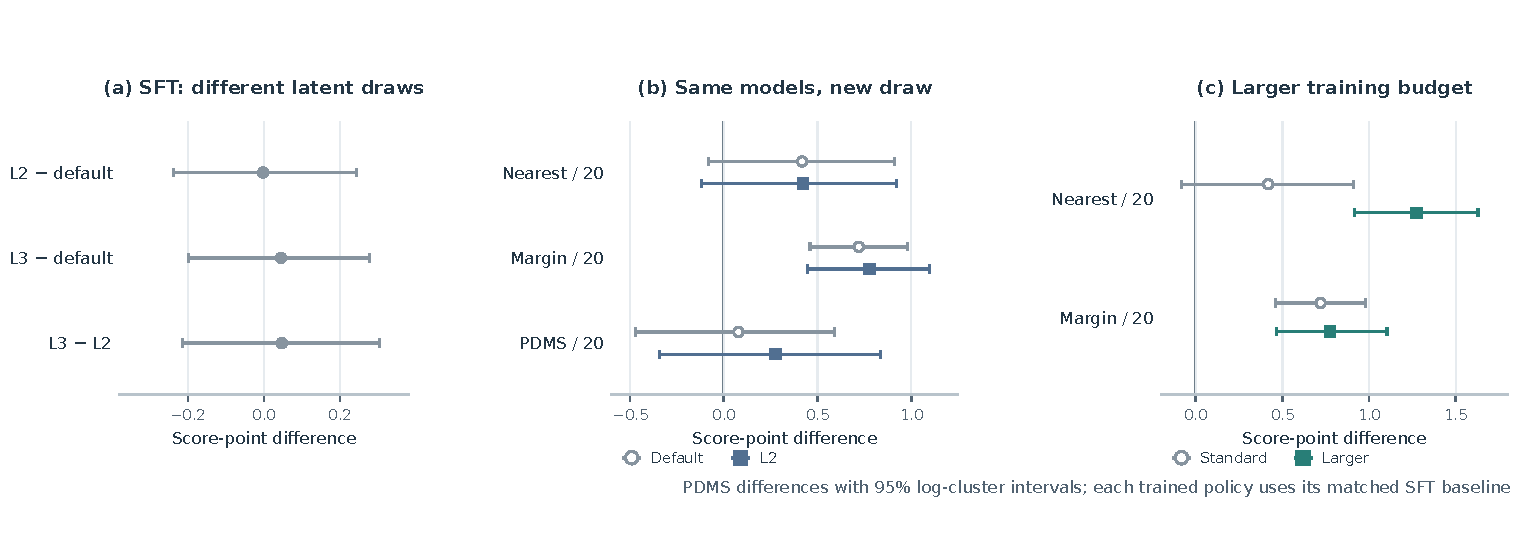
\includegraphics[width=0.85\linewidth]{figures/ral/fig4_sampling_budget.pdf}
\caption{\textbf{Checks beyond one inference draw and budget.} (a) SFT contrasts across initial latent draws. (b) Fixed seed-20 policies under two draws, each versus matching SFT. (c) Standard versus larger training budgets at seed 20, each versus SFT. Bars are 95\% log-cluster intervals for the displayed differences, not for differences between conditions. The larger budget changes both scenes and updates.}
\label{fig:sampling_budget}
\end{figure}

\FloatBarrier
\section{Progress-capped ablation and target statistics}
\begin{table}[H]
\centering\caption{Progress-capped score rule, full navtest, against SFT (86.99). R/N: repairs/new failures. The capped pair file has 860 of the 988 standard pairs.}
\small\setlength{\tabcolsep}{3pt}
\begin{tabular}{lrrrrr}\toprule
Seed & $\Delta$PDMS [95\% interval] & NC R/N & DAC R/N & TTC R/N & Net\\\midrule
20 & $-0.024$ [$-0.778$,0.689] & 68/44 & 196/177 & 182/79 & +146\\
21 & +0.441 [$-0.177$,0.999] & 78/28 & 179/119 & 207/49 & +268\\
22 & +0.432 [0.051,0.796] & 66/17 & 144/80 & 177/31 & +259\\
23 & +0.852 [0.484,1.200] & 53/17 & 141/42 & 167/28 & +274\\\bottomrule
\end{tabular}
\end{table}
Progress against SFT is $-1.102$ [$-1.764$,$-0.514$], $-0.966$ [$-1.506$,$-0.491$], $-0.922$ [$-1.273$,$-0.603$], and $-0.210$ [$-0.537$,0.103]. Against the uncapped PDMS policy of the same seed, $\Delta$PDMS is $-0.103$ [$-0.468$,0.237], +1.312 [0.833,1.823], +0.685 [0.253,1.156], and +1.001 [0.577,1.440], with TTC differences of +1.498, +2.766, +2.272, and +1.828. Against nearest-reference the capped policy is lower at seeds 20--22 and unresolved at seed 23; against maximum margin it is lower at seeds 20 and 22, unresolved at seed 21, and higher at seed 23 (+0.457 [0.114,0.830]).

\begin{table}[H]
\centering\caption{Selected training targets. Clearance is the recorded minimum agent clearance; displacement is the mean planar waypoint distance from the mean reference-probe trajectory; progress is relative to the reference's mean progress. Clearance is expressed in meters and progress differences in score points. The capped row uses a different subset; this table describes targets, while the random-winner policy outcomes are reported below.}
\small\setlength{\tabcolsep}{3pt}
\begin{tabular}{lrrrrr}\toprule
Rule & Pairs & Clearance (m) & $\Pr[c\le 2.5\,\mathrm m]$ & Displ.\ (m) & $\Delta$EP\\\midrule
PDMS & 988 & 4.19 & 0.563 & 0.420 & +10.6\\
Maximum margin & 988 & 4.56 & 0.508 & 0.385 & +8.4\\
Nearest reference & 988 & 4.19 & 0.563 & 0.084 & +8.6\\
Random eligible & 988 & 4.22 & 0.561 & 0.284 & +8.6\\
PDMS, progress-capped & 860 & 4.12 & 0.572 & 0.223 & $-0.1$\\\bottomrule
\end{tabular}
\end{table}
\subsection{Random eligible winners: three completed training seeds}
We sample one winner uniformly from each eligible set, using the same training scenes and with the same loser construction and fitting recipe. One fixed selection seed defines the target set; training seeds 20--22 vary policy fitting, not the target-set draw. Their v1 gains over SFT are +0.54, +0.59, and +0.71, and same-seed gains over PDMS are +0.46 [0.07,0.84], +1.46 [1.02,1.96], and +0.96 [0.67,1.30].

\begin{table}[H]
\centering
\caption{Random-winner contrasts on full navtest. All trained-rule comparisons use seeds 20--22 and per-scene seed means. Intervals condition on the fitted policies.}
\begin{tabular}{lrrrrr}\toprule
Contrast & Total [95\% interval] & NC & DAC & TTC & EP\\\midrule
Random $-$ SFT & +0.61 [0.14,1.04] & +0.23 & +0.48 & +0.70 & +0.10\\
Random $-$ PDMS & +0.96 [0.63,1.30] & +0.53 & +0.88 & +1.76 & $-0.82$\\
Random $-$ nearest & $-0.11$ [$-0.29$,0.05] & $-0.09$ & $-0.20$ & $-0.31$ & +0.31\\
Random $-$ margin & $-0.07$ [$-0.23$,0.08] & $-0.09$ & $-0.18$ & $-0.25$ & +0.33\\\bottomrule
\end{tabular}
\end{table}
The unresolved total-score contrasts do not establish equivalence. Geometry retains safety-component advantages, while the random control has higher progress. These results concern one sampled target set. They show that explicit geometric ranking is not required for the observed improvement over score selection, not that every passing target is equally useful. The geometric comparisons use the same three seeds as the random control. A missing total-score difference is not evidence that the two supervision rules are interchangeable across safety and progress.

\subsection{Approximation error on training scenes}
On 300 shared training scenes, we pair each selected winner with one policy output from a fixed scene-specific latent and deterministic ten-step integration. The base and fitted policies use the same latent; the stored winner need not have been generated from that latent. This defines a same-scene target--output pairing, not an optimal coupling. Table~\ref{tab:epsw} reports $\hat\epsilon_w=\sqrt{\text{mean}\|\widehat A-A^+\|^2}$ over the normalized 24-dimensional relative-action vectors. We also report $\delta_{xy}$, the mean planar error in the eight \emph{relative action increments}, after undoing normalization. Its units are meters, but it is not an error between integrated waypoint positions. Both measurements compare the base policy and the seed-20 fitted policy to each rule's targets.

\begin{table}[H]
\centering
\caption{Distance between policy output and the selected winner on 300 shared training scenes. Entries report $\hat\epsilon_w$ in normalized relative-action space / mean planar increment error $\delta_{xy}$ in meters. These are training-scene diagnostics, not a calibrated safety bound.}
\label{tab:epsw}
\begin{tabular}{lcc}
\toprule
Winner rule & Base policy & Fitted (seed 20) \\
\midrule
PDMS & 0.246 / 0.135 & 0.245 / 0.123 \\
Margin & 0.240 / 0.112 & 0.250 / 0.116 \\
Nearest & 0.203 / 0.082 & 0.214 / 0.096 \\
\bottomrule
\end{tabular}
\end{table}

Fitting changes the aggregate errors only slightly. The normalized error increases for margin and nearest-reference and is nearly unchanged for PDMS. Margin and PDMS also have similar fitted increment errors (0.116 and 0.123\,m), despite opposite repair balances. Thus these summaries do not explain the rule ordering. They leave error tails, their alignment with constraint boundaries, and held-out generalization unresolved. In particular, a small relative-action error does not establish small integrated trajectory error or preserved simulator feasibility. Connecting this diagnostic to the main paper's conditional feasibility bound requires a constraint margin and Lipschitz constant in the same action representation.


\FloatBarrier
\section{V2 scorer sensitivity}
Saved trajectories of SFT, twelve standard policies, and four capped policies were re-scored on all 12,146 scenes using the v2 one-stage scorer under non-reactive traffic and reactive IDM agents. Scores are averaged across four seeds within each scene before paired log resampling. This reuses trained policies and scenes; it is not an independent replication, closed-loop policy execution, or the complete two-stage v2 pseudo-simulation benchmark.
\begin{table}[H]
\centering\caption{V2 total-score contrasts of four-seed per-scene means, with 95\% paired log-cluster intervals.}
\begin{tabular}{lcc}\toprule
Contrast & Non-reactive & Reactive IDM\\\midrule
Margin $-$ PDMS & +0.406 [0.038,0.802] & +0.591 [0.276,0.956]\\
Nearest $-$ PDMS & +0.514 [0.117,0.945] & +0.660 [0.298,1.050]\\
Capped $-$ PDMS & +0.114 [$-0.204$,0.459] & +0.268 [$-0.022$,0.580]\\
PDMS $-$ SFT & $-0.300$ [$-0.947$,0.288] & $-0.532$ [$-1.145$,0.043]\\\bottomrule
\end{tabular}
\end{table}
The geometric-versus-score advantage persists, but no rule has a resolved v2 total-score gain over SFT. All four training rules lose 0.55--0.67 lane-keeping points with intervals below zero. These outcomes support relative rule comparisons, not comprehensive improvement. Multi-Anchor results concern ranking rather than transfer of the post-training intervention across decoders.


\end{document}
